
If an matrix style display is used with a microcontroller, there are a lot of different ways to draw graphical elements. This chapter \ref{chapter:DrawGraph} covers only the ways used in this project. 

\subsubsection{Matrix displays}

Since most displays produced have an rectangular shape the amount of pixel they hold is calculated like the surface of an rectangular. The number of pixels on both axis are multiplied and we get the total amount of pixels we have to manipulate. So it is obvious that the memory size of an picture explodes with its resolution. As an example we take a display with a pixel ratio of 1200 x 825 and a colour depth of 24 bit. We get $1200\cdot825=990'000$ pixel and $1200\cdot825\cdot24=23'760'000$ bits we have to handle. This is a huge amount of data to process with a microcontroller.\\
If an display is rectangular the information of the pixels can be ordered in a matrix. The matrix is normally one or two dimensions.  

\begin{figure}[H]
	\centering
	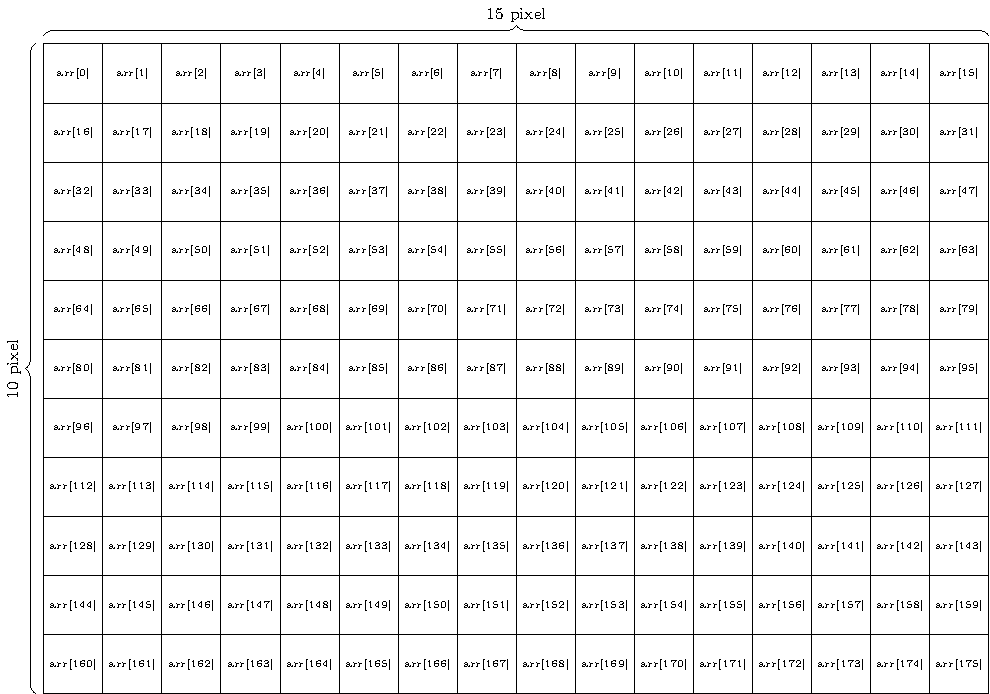
\includegraphics[width=1\textwidth]{2-theory/drawing-graphics/graphics/matrix.pdf}
	\caption{One level display matrix \label{theory:matrix}}
\end{figure}

\begin{figure}[H]
	\centering
	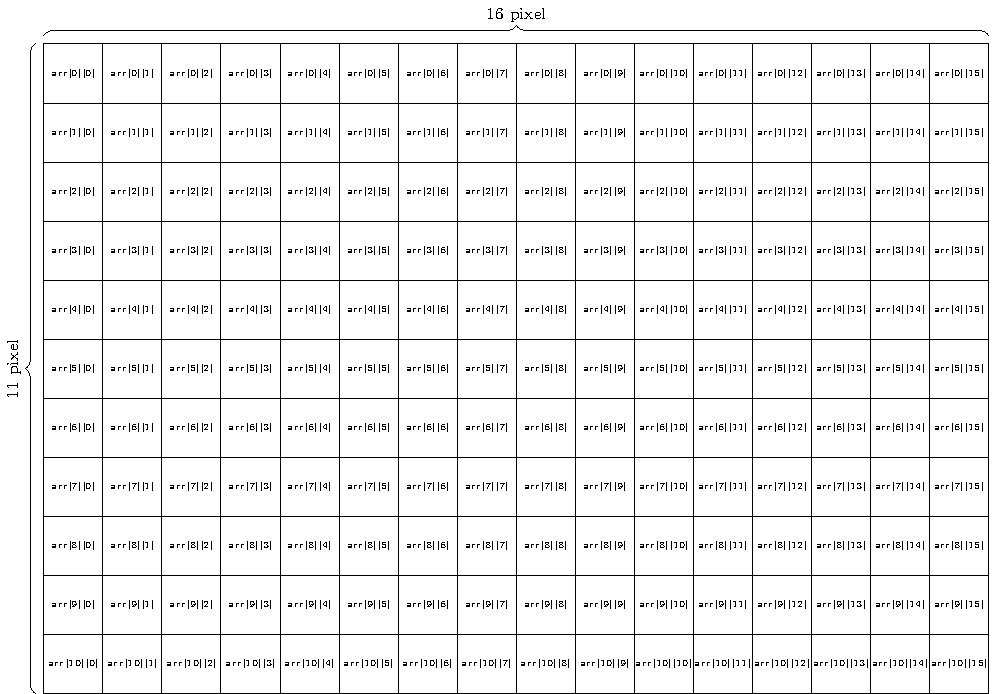
\includegraphics[width=1\textwidth]{2-theory/drawing-graphics/graphics/matrix2.pdf}
	\caption{Two level display matrixl\label{theory:matrix2}}
\end{figure}

\subsubsection{Double buffering}


  

\begin{figure}[H]
	\centering
	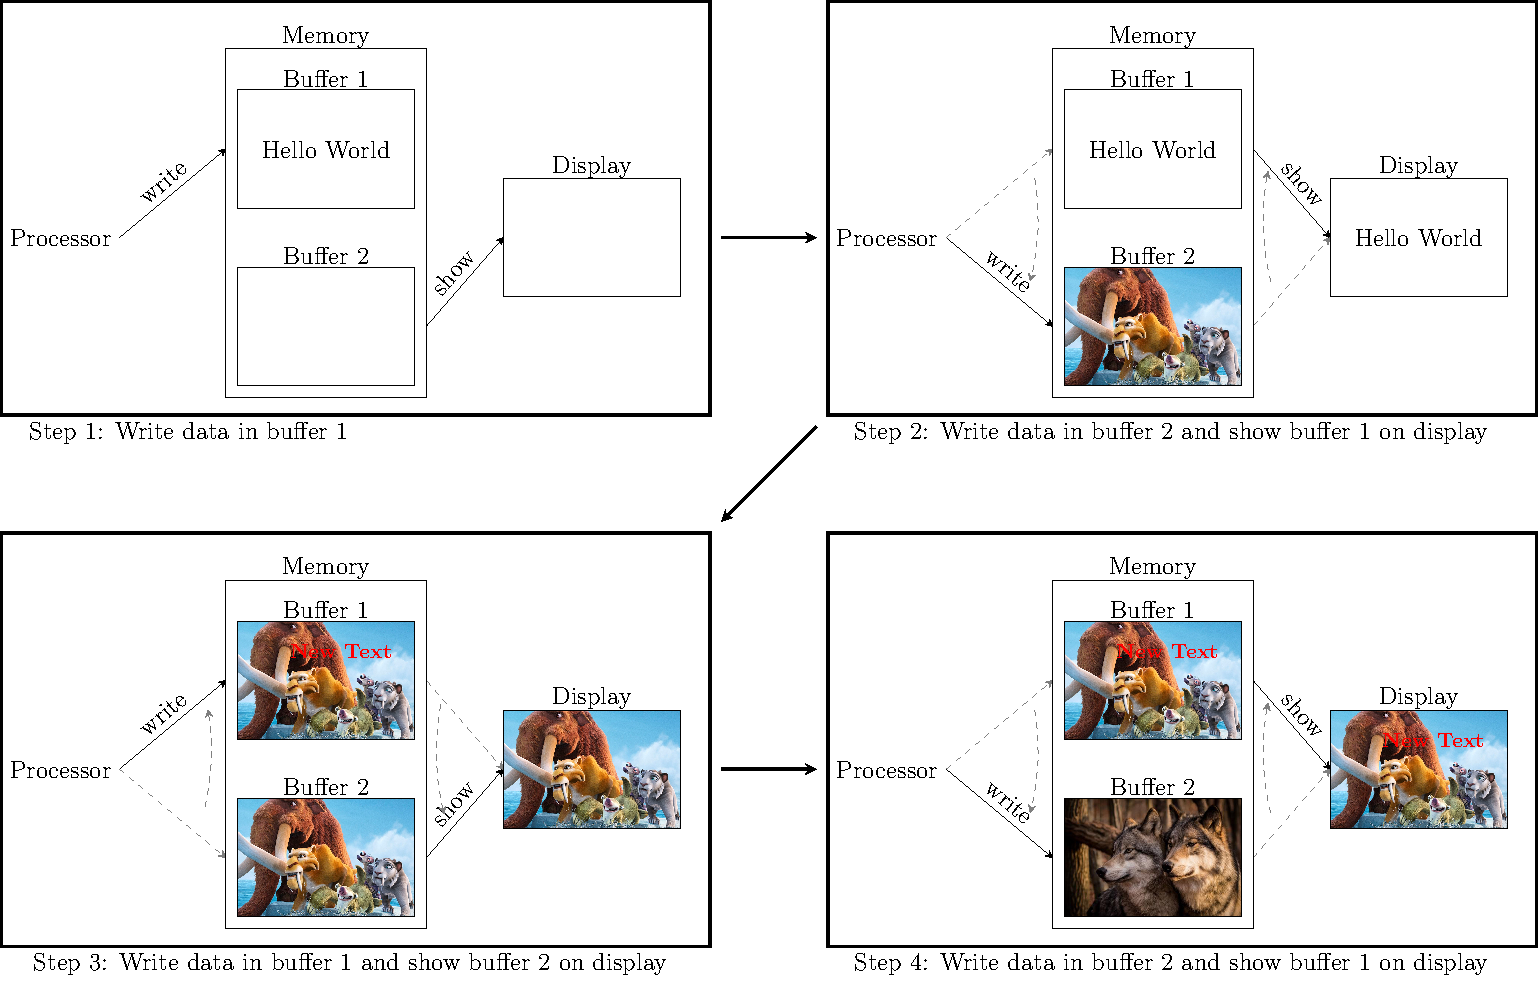
\includegraphics[width=1\textwidth]{2-theory/drawing-graphics/graphics/buffer.pdf}
	\caption{Double buffer example while writing different images to screen\label{theory:buffer}}
\end{figure}




\subsubsection{Compressed fonts}\label{chapter:CompressedFonts}

The theory shown in this chapter \ref{chapter:CompressedFonts} is only valid if the fonts used are simple fonts which are using only two different values. More complex fonts have to be compressed in a different way to avoid data loss. 
\begin{figure}[H]
	\centering
	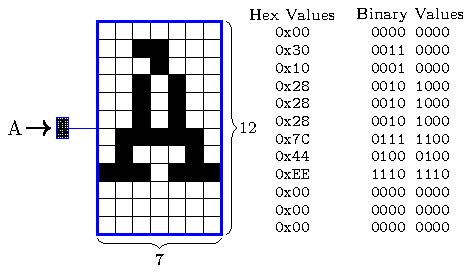
\includegraphics[width=0.8\textwidth]{2-theory/drawing-graphics/graphics/font12.pdf}
	\caption{Creation of a simple seven to twelve pixel sized font\label{theory:font12}}
\end{figure}



\subsection{Drawing text to the display}